\documentclass{ieeeaccess}

\usepackage{cite}
\usepackage[T1]{fontenc}
\usepackage[utf8]{inputenc}
\usepackage{xcolor}
\usepackage{amsmath,amssymb,amsfonts,amsthm}
\usepackage{algorithm}
\usepackage{algpseudocode}
\usepackage{graphicx}
\usepackage{textcomp}
\usepackage{booktabs,array}
\usepackage{url}
\usepackage{microtype}
\usepackage{balance}
\usepackage[hidelinks,breaklinks]{hyperref}

\xdef\xfigwd{0pt}% lets the class wrap long figure captions
\newcommand{\fillin}[1]{{\color{red}[#1]}}

\newtheorem{theorem}{Theorem}
\newtheorem{lemma}{Lemma}
\newtheorem{definition}{Definition}

\newcommand{\Pfree}{P_{\mathrm{free}}}
\newcommand{\dfree}{d_{\mathrm{free}}}
\DeclareMathOperator{\pos}{pos}
\newcommand{\ind}{\mathbf{1}}
\newcommand{\Lin}{\mathcal{L}}

\begin{document}
\vol{12}
\year{2026}
\history{}
\doi{To be assigned after acceptance}

\title{Counterfactual Flip-Cost Analysis: Quantifying Pairwise Ordering Ambiguity in Precedence-Constrained Security Timelines}

\author{KAMALESH N.$^{1}$, AND VARUN DUBEY$^{1}$}

\address[1]{School of Computer Science and Engineering, Vellore Institute of Technology, Chennai Campus, Chennai 600127, Tamil Nadu, India (e-mail: kamalesh.n2024@vitstudent.ac.in, varun.dubey2024@vitstudent.ac.in)}

\corresp{Corresponding author: Kamalesh N. (e-mail: kamalesh.n2024@vitstudent.ac.in).}

\begin{abstract}
Reconstructing attack timelines from heterogeneous security logs is undermined by timestamp distortion: per-core clock skew, network latency, coarse quantisation, and deliberate anti-forensic timestomping. Provenance and domain causality supply invariant precedence constraints, a directed acyclic graph (DAG) whose linear extensions are the admissible timelines, but choosing the extension closest to the recorded timestamps is the Nearest-Neighbour Kendall-Tau Distance problem, which is NP-complete. A single optimal timeline hides how fragile each ordering decision is. We introduce the \emph{counterfactual flip-cost} $\Delta(a,b)$: the extra reconstruction cost of forcing two unconstrained events to occur in reverse order, and we prove it equals the scaled log-ratio of extremal maximum-a-posteriori (MAP) realizations of a precedence-conditioned Mallows model. Unlike process-mining estimators, it needs only one incident, with no case library. We compute it with a budget-bounded A* search with an admissible heuristic and exact subset-dominance pruning (matching brute force on 60/60 instances), and we add farthest-first selection to expose structurally distinct near-optimal timelines. On synthetic DAGs, flip-cost reaches pairwise AUROC 0.801--0.856 under Gaussian jitter and 0.835 under multi-host clock skew, against 0.583--0.605 for a Mallows-marginal baseline. It is statistically indistinguishable from a timestamp-margin heuristic at $\sigma\le2$\,s and significantly better at $\sigma=4$\,s ($+0.061$, 95\% CI $[+0.030,+0.092]$). Flip-based diversity selection raises free-pair diversity from 0.060 to 0.145 at about four times the search cost. Evaluation is synthetic only; validation on operational logs remains future work.
\end{abstract}

\begin{keywords}
Counterfactual analysis, digital forensics, heuristic search, incident timeline reconstruction, Kendall-tau distance, linear extensions, ordering ambiguity, partial orders.
\end{keywords}

\titlepgskip=-15pt

\maketitle

%=====================================================================
\section{Introduction}\label{sec:intro}
\PARstart{S}{ecurity} event logs generated by enterprise endpoints, firewalls, operating-system audit daemons, and cloud infrastructure are the primary forensic foundation for triage, root-cause analysis, and attack-scenario reconstruction in Security Operations Centers (SOCs) \cite{Hossain2017,Cheng2024}. During incident response, analysts must reconstruct a chronological \emph{timeline} to establish the adversary's initial vector, privilege-escalation pathway, and exfiltration sequence.

Treating recorded timestamps as ground truth is, however, hazardous. Three distortion vectors are pervasive:
\begin{enumerate}
\item \textbf{Clock asynchrony and drift.} NTP drift, hypervisor pauses, and hardware differences introduce jitter across hosts, and unsynchronized per-core counters yield non-monotonic timestamps even within one host. Kimm \emph{et al.} \cite{Kimm2026} measured that 3.0\%--3.5\% of audit records are logged out of order solely due to multi-core timestamp drift.
\item \textbf{Coarse quantisation.} Commercial off-the-shelf (COTS) logging such as Windows EVTX and Syslog records events at millisecond or second granularity, collapsing sequential operations onto identical timestamps.
\item \textbf{Adversarial manipulation.} Attackers apply anti-forensic \emph{timestomping}, deliberately rewriting file-system and log timestamps to disrupt chronological reconstruction \cite{Peisert2007}.
\end{enumerate}
Kernel-level atomic sequence numbers (e.g., via eBPF or \texttt{auditd}) can totally order events within a single kernel stream \cite{Kimm2026}, but they cannot be retrofitted to legacy COTS logs or applied when fusing evidence across firewalls, web servers, and directory services during multi-host lateral movement.

Without trustworthy timestamps, investigators must lean on \emph{domain causality and provenance constraints} \cite{Hossain2017,Cheng2024,King2003,Pasquier2017}: a file cannot be read before it is created, and a child process cannot run before its parent forks. These invariant dependencies form a Directed Acyclic Graph (DAG) $G=(V,E)$ that defines a partially ordered set (poset) of events \cite{Pegoraro2020a}. Every admissible timeline is a \emph{linear extension} (topological sort) of this poset; we write $\Lin(G)$ for the set of all of them. When $E$ does not determine all pairs, $|\Lin(G)|$ can grow exponentially, and counting it is $\#$P-complete \cite{Brightwell1991}. Selecting the extension that minimizes disagreement with the recorded timestamps is the Nearest-Neighbour Kendall-Tau Distance problem, which is NP-complete \cite{Brandenburg2011}.

\emph{Contrast with process mining.} Partial-order resolution in process mining \cite{vanderAa2020,Pegoraro2020a,Pegoraro2021} estimates probability distributions over total orders from hundreds or thousands of repeated executions of structured business processes. Cyber attacks are rare, one-off events: no historical case base of repeated executions exists, so such estimators have nothing to learn from in a single-incident investigation.

\emph{Our approach.} A single best timeline conceals fragility: two independent events whose timestamps differ by milliseconds will be ordered one way, and an analyst may build a containment theory on that arbitrary choice. We therefore ask a counterfactual question for each unconstrained pair $(a,b)$ ordered $a\prec b$ in the optimum $\pi^*$: \emph{what is the minimum additional cost of forcing $b$ before $a$?} This defines the \textbf{Counterfactual Flip-Cost}
\begin{equation}
\Delta(a,b)=c_{\mathrm{flip}}(a,b)-c(\pi^*),
\end{equation}
which we prove equals the scaled log-ratio of extremal Maximum A Posteriori (MAP) realizations of a precedence-conditioned Mallows model \cite{Mallows1957,Lu2011}.

Fig.~\ref{fig:concept} illustrates the idea on a five-event example.

\begin{figure*}[!t]
\centering
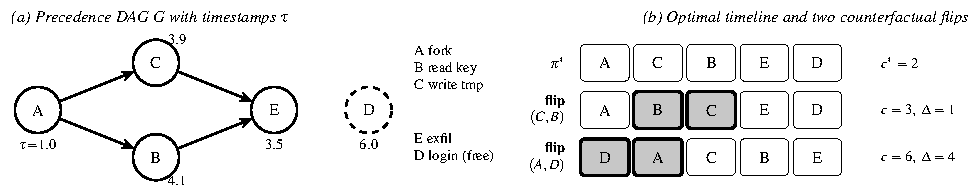
\includegraphics[width=\textwidth]{figures/concept.pdf}
\caption{Counterfactual flip-cost on a five-event example (all values verified by exhaustive enumeration of the 10 linear extensions). (a) Fork A must precede both B and C, which must precede exfiltration E; login D is unconstrained. Recorded timestamps are distorted: E appears before B and C. (b) The optimum $\pi^*$ has Kendall-tau cost $c^*=2$. Reversing the pair $(C,B)$ costs only $\Delta=1$: its order is \emph{fragile}, and the 0.2\,s timestamp gap agrees. Reversing $(A,D)$ forces $D$ to the front and costs $\Delta=4$: its order is \emph{robust}. Shaded cells mark the swapped events.}
\label{fig:concept}
\end{figure*}

The contributions of this paper are:
\begin{enumerate}
\item \textbf{Theoretical grounding.} We formalize timeline ambiguity as constrained Kendall-tau minimization on posets, establish hardness via \cite{Brandenburg2011}, and prove that $\Delta(a,b)$ is the log-ratio of extremal MAP values of a conditioned Mallows model.
\item \textbf{Flip-cost metric and algorithm.} We define the bounded flip-cost $\Delta_B(a,b)$ with an explicit unverified status $\bot$, and give a budget-bounded A* search with an admissible heuristic and exact subset-dominance pruning.
\item \textbf{Diversity-aware selection.} We propose farthest-first candidate selection over unconstrained pairs $\Pfree$ to expose structurally distinct near-optimal timelines.
\item \textbf{Empirical evaluation.} We benchmark on synthetic DAGs under Gaussian jitter and a structured multi-host clock-skew model, with paired bootstrap confidence intervals, scalability to 50 events, and comparison against margin and Mallows-marginal baselines.
\end{enumerate}

The remainder of the paper is organized as follows. Section~\ref{sec:related} reviews related work. Section~\ref{sec:problem} formalizes the problem and theory. Section~\ref{sec:method} presents the methodology. Section~\ref{sec:setup} describes the experimental setup, Section~\ref{sec:results} reports results, Section~\ref{sec:threats} discusses validity threats, and Section~\ref{sec:conclusion} concludes.

%=====================================================================
\section{Related Work}\label{sec:related}

\subsection{Partial-Order Resolution in Event Logs and Process Mining}
When timestamps overlap or recording clocks are unsynchronized, a trace generalizes from a sequence to a partial order \cite{vanderAa2020,Pegoraro2020a}. Pegoraro \emph{et al.} \cite{Pegoraro2020a,Pegoraro2020b} introduced behavior graphs for uncertain event data, adding an edge only when two timestamp-uncertainty intervals do not overlap; this preserves only indisputable precedences but neither ranks the resulting linear extensions nor measures the sensitivity of any ordering decision. van der Aa \emph{et al.} \cite{vanderAa2020} resolve partial orders for conformance checking by estimating a distribution over total orders from behavioral abstractions across a large historical log, and Pegoraro \emph{et al.} \cite{Pegoraro2021} estimate probabilities of uncertain trace realizations. These \emph{cross-case trace-distribution estimators} require a repeated process. Our metric is instead a \emph{single-incident, deterministic, extremal} sensitivity measure computed from one DAG and one set of timestamps.

\subsection{Combinatorial Complexity of Posets and Linear Extensions}
Brightwell and Winkler \cite{Brightwell1991} proved that counting linear extensions is $\#$P-complete; Dittmer and Pak \cite{Dittmer2020} showed hardness persists for restricted posets, and exact dynamic programming over ideals \cite{Kangas2016} remains exponential in general. Huber \cite{Huber2006} gave perfect uniform sampling of linear extensions, but uniform sampling ignores timestamp evidence. Brandenburg \emph{et al.} \cite{Brandenburg2011} formalized the Nearest-Neighbour Kendall-Tau Distance between a partial order and a total order, proved NP-completeness by reduction from One-Sided Crossing Minimization on 4-stars (OSCM-4-Star), and gave a 2-approximation. The problem is closely related to precedence-constrained feedback-arc-set ranking, for which van Zuylen and Williamson \cite{vanZuylen2009} give deterministic pivoting algorithms and Mastrolilli \cite{Mastrolilli2011} studies the triangle-inequality case. Our work builds on these hardness results to motivate budget-bounded exact search.

\subsection{Diverse Top-$K$ Optimization and Heuristic Search}
Classical $K$-best methods such as Eppstein's algorithm \cite{Eppstein1998} and $K^*$ \cite{Aljazzar2011} return the $K$ cheapest solutions, which in permutation problems cluster around trivial local swaps. Batra \emph{et al.} \cite{Batra2012} add a dissimilarity term to the objective for diverse $M$-best MRF solutions; Sohrabi \emph{et al.} \cite{Sohrabi2016} generate a pool of plans and cluster it for hypothesis generation; Katz \emph{et al.} \cite{Katz2020,Katz2022} formulate top-quality and quality-bounded diverse planning. Lepsien \emph{et al.} \cite{Lepsien2024} rank top-$K$ realizations of stochastic event logs, but address stochastic activity-label uncertainty under independence rather than structural ordering ambiguity under DAG constraints. We adopt a two-phase pool-then-diversify design in the spirit of \cite{Sohrabi2016,Katz2020}, with distance measured on $\Pfree$.

\subsection{Cyber Provenance, Audit Asynchrony, and Counterfactual Reasoning}
Provenance-based systems such as SLEUTH \cite{Hossain2017} and KAIROS \cite{Cheng2024}, building on BackTracker \cite{King2003} and whole-system provenance capture \cite{Pasquier2017}, convert audit records into causal graphs for attack investigation. Kimm \emph{et al.} \cite{Kimm2026} showed multi-core audit skew produces out-of-order records and repair it with kernel-attached global sequence numbers, which cannot be retrofitted to legacy or multi-host data. Wachter \emph{et al.} \cite{Wachter2018} defined counterfactual explanations as minimal input perturbations that change a decision; analogously, $\Delta(a,b)$ is the minimal objective perturbation needed to invert a pairwise temporal relation. Table~\ref{tab:taxonomy} summarizes the positioning.

\begin{table*}[!t]
\caption{Taxonomic Positioning of the Proposed Framework}
\label{tab:taxonomy}
\centering
\footnotesize
\setlength{\tabcolsep}{3pt}
\renewcommand{\arraystretch}{1.15}
\begin{tabular}{@{}>{\raggedright\arraybackslash}p{2.6cm}>{\raggedright\arraybackslash}p{1.8cm}>{\raggedright\arraybackslash}p{2.5cm}>{\raggedright\arraybackslash}p{2.9cm}>{\raggedright\arraybackslash}p{3.1cm}>{\raggedright\arraybackslash}p{2.3cm}>{\raggedright\arraybackslash}p{1.9cm}@{}}
\toprule
\textbf{Framework} & \textbf{Domain} & \textbf{Input constraints} & \textbf{Primary objective} & \textbf{Sensitivity metric} & \textbf{Diversity mechanism} & \textbf{Case base required?}\\
\midrule
van der Aa \emph{et al.} \cite{vanderAa2020} & Process mining & Partial-order traces & Trace conformance likelihood & Global trace probability distribution & None & Yes (cross-case log)\\
Pegoraro \emph{et al.} \cite{Pegoraro2020a} & Process mining & Timestamp intervals & Behavior-graph DAG construction & None (encodes feasible orders only) & None & No\\
SLEUTH / KAIROS \cite{Hossain2017,Cheng2024} & Cyber forensics & OS provenance DAG & Attack-graph reachability and triage & None & Single graph summary & No\\
Kimm \emph{et al.} \cite{Kimm2026} & System auditing & Per-core OS audit logs & Causal provenance repair & None (deterministic sequence-ID repair) & Single total order & No (needs custom kernel/eBPF)\\
Batra \emph{et al.}; Katz \emph{et al.} \cite{Batra2012,Katz2020} & AI planning / MRF & State-transition rules & Cost-bounded plan generation & None (plan quality only) & In-search / top-quality diversity & No\\
Brandenburg \emph{et al.} \cite{Brandenburg2011} & Theoretical CS & Poset + reference order & Nearest-neighbour Kendall-tau & None (2-approximation) & None & No\\
\midrule
\textbf{Proposed framework} & \textbf{Cyber forensics} & \textbf{Causal DAG + noisy timestamps} & \textbf{Nearest-neighbour Kendall-tau linear extension} & \textbf{Pairwise counterfactual flip-cost $\Delta(a,b)$ (MAP log-ratio)} & \textbf{Farthest-first over $\Pfree$} & \textbf{No (single incident)}\\
\bottomrule
\end{tabular}
\end{table*}

\emph{Research gap.} Prior work builds precedence DAGs \cite{Pegoraro2020a}, repairs single-host sequences \cite{Kimm2026}, or estimates trace distributions over many executions \cite{vanderAa2020}. None provides an objective-relative, single-incident measure of how easily an individual decision $a\prec b$ can be overturned.

%=====================================================================
\section{Problem Formulation and Theoretical Foundations}\label{sec:problem}

\subsection{Definitions}
Let $V=\{v_1,\dots,v_n\}$ be the observed events, each with a recorded timestamp $\tau(v)\in\mathbb{R}^+$. Let $\pi_\tau$ be the \emph{reference sequence} obtained by sorting $V$ by non-decreasing $\tau$, ties broken by a deterministic rule (lexicographic event identifier).

\begin{definition}[Precedence DAG and poset]
$G=(V,E)$ is a DAG in which $(u,v)\in E$ requires $u$ to occur before $v$. Its transitive closure $E^+$ induces the strict partial order $u\prec_G v \iff (u,v)\in E^+$.
\end{definition}

\begin{definition}[Valid timeline]
A timeline is a bijection $\pi:\{1,\dots,n\}\to V$ with $\pos_\pi(v)$ the 1-indexed position of $v$. It is \emph{valid} iff $\pos_\pi(u)<\pos_\pi(v)$ for all $(u,v)\in E$. The set of valid timelines is the set of linear extensions $\Lin(G)$.
\end{definition}

\begin{definition}[Free pairs]
\begin{equation}
\Pfree=\{(u,v)\mid u\neq v,\ (u,v)\notin E^+,\ (v,u)\notin E^+\}.
\end{equation}
If $\Pfree=\emptyset$ then $|\Lin(G)|=1$ and there is no ordering ambiguity.
\end{definition}

\subsection{Kendall-Tau Inversion Cost}
Because timestamps are noisy, $\pi_\tau\notin\Lin(G)$ in general. The reconstruction cost of $\pi$ is its Kendall-tau distance \cite{Kendall1938} to $\pi_\tau$:
\begin{multline}
c(\pi)=\sum_{1\le i<j\le n}\ind\!\big[(\pos_{\pi_\tau}(v_i)-\pos_{\pi_\tau}(v_j))\\
\cdot(\pos_\pi(v_i)-\pos_\pi(v_j))<0\big].
\end{multline}
The baseline problem is $\pi^*\in\arg\min_{\pi\in\Lin(G)}c(\pi)$, with $c^*=c(\pi^*)$.

\subsection{Computational Complexity}
\begin{theorem}[NP-completeness]\label{thm:np}
Given $G$, $\pi_\tau$, and an integer $K\ge 0$, deciding whether some $\pi\in\Lin(G)$ has $c(\pi)\le K$ is NP-complete.
\end{theorem}
\begin{proof}
The problem is exactly the Nearest-Neighbour Kendall-Tau Distance between a partial order and a total order. Brandenburg \emph{et al.} \cite{Brandenburg2011} prove NP-hardness by polynomial-time reduction from OSCM-4-Star. Membership in NP holds because a certificate $\pi$ is verified by checking all edges of $E$ and evaluating $c(\pi)$ in $O(|V|+|E|+|V|^2)$ time.
\end{proof}

\begin{theorem}[Counting intractability]\label{thm:sharpp}
Computing $|\Lin(G)|$ is $\#$P-complete.
\end{theorem}
\begin{proof}
This is the theorem of Brightwell and Winkler \cite{Brightwell1991}; hardness persists for posets of height two \cite{Dittmer2020}.
\end{proof}

Theorems~\ref{thm:np} and~\ref{thm:sharpp} preclude exhaustive enumeration and motivate a budget-bounded best-first search with admissible pruning.

\subsection{Conditioned Mallows Model and the MAP Log-Ratio}
The Mallows model \cite{Mallows1957} centered at $\pi_\tau$ with dispersion $\theta>0$ assigns $P(\pi\mid\pi_\tau,\theta)\propto\exp(-\theta\,c(\pi))$ over all permutations \cite{Lu2011}. Provenance constraints are deterministic evidence: any $\pi\notin\Lin(G)$ is impossible. Conditioning on $G$ gives
\begin{equation}
P(\pi\mid G)=\frac{1}{Z_G(\theta)}\exp(-\theta\,c(\pi))\cdot\ind[\pi\in\Lin(G)],
\end{equation}
with $Z_G(\theta)=\sum_{\pi\in\Lin(G)}\exp(-\theta c(\pi))$.

For $(a,b)\in\Pfree$ with $a\prec b$ in $\pi^*$, let $\Lin_{\mathrm{flip}}(a,b)$ be the linear extensions with $\pos(b)<\pos(a)$. This is precisely $\Lin(G_{\mathrm{flip}})$ for $G_{\mathrm{flip}}=(V,E\cup\{(b,a)\})$, which is acyclic because $(a,b)\in\Pfree$. Define $c_{\mathrm{flip}}(a,b)=\min_{\pi\in\Lin_{\mathrm{flip}}(a,b)}c(\pi)$.

\begin{theorem}[Equivalence to extremal MAP log-ratio]\label{thm:map}
For every $(a,b)\in\Pfree$ and $\theta>0$,
\begin{equation}
\Delta(a,b)=c_{\mathrm{flip}}(a,b)-c^*=\frac{1}{\theta}\ln\!\left[\frac{\max_{\pi\in\Lin(G)}P(\pi\mid G)}{\max_{\pi\in\Lin_{\mathrm{flip}}(a,b)}P(\pi\mid G)}\right].
\end{equation}
\end{theorem}
\begin{proof}
Fix a nonempty $\Lin'\subseteq\Lin(G)$. Since $Z_G(\theta)$ does not depend on $\pi$ and $x\mapsto e^{-\theta x}$ is strictly decreasing for $\theta>0$,
\begin{equation}
\max_{\pi\in\Lin'}P(\pi\mid G)=\frac{1}{Z_G(\theta)}\exp\!\Big(-\theta\min_{\pi\in\Lin'}c(\pi)\Big).
\end{equation}
$\Lin_{\mathrm{flip}}(a,b)\neq\emptyset$ because $(a,b)\in\Pfree$ implies $G_{\mathrm{flip}}$ is acyclic and thus has a topological order. Applying the display to $\Lin'=\Lin(G)$ (minimum $c^*$) and to $\Lin'=\Lin_{\mathrm{flip}}(a,b)$ (minimum $c_{\mathrm{flip}}$), the common factor $1/Z_G(\theta)$ cancels:
\begin{equation}
\frac{\max_{\Lin(G)}P}{\max_{\Lin_{\mathrm{flip}}}P}=\frac{e^{-\theta c^*}}{e^{-\theta c_{\mathrm{flip}}(a,b)}}=e^{\theta\,(c_{\mathrm{flip}}(a,b)-c^*)}.
\end{equation}
Taking $\ln$ and dividing by $\theta>0$ yields $\Delta(a,b)$.
\end{proof}

\subsection{Extremal Flip-Cost versus Marginal Probability}
The marginal probability of reversal integrates over \emph{all} extensions,
\begin{equation}
P(b\prec a\mid G)=\frac{Z_{\mathrm{flip}}(\theta)}{Z_G(\theta)}=\frac{\sum_{\pi\in\Lin_{\mathrm{flip}}}e^{-\theta c(\pi)}}{\sum_{\pi\in\Lin(G)}e^{-\theta c(\pi)}},
\end{equation}
and requires two $\#$P-hard partition functions, making it sensitive to the sheer volume of sub-optimal permutations. In contrast, $\Delta(a,b)$ is an \emph{extremal} (MAP) measure: $\Delta=0$ means an equally consistent timeline places $b$ before $a$, so the decision $a\prec b$ is arbitrary, while $\Delta\gg0$ means reversal forces severe temporal incoherence.

\subsection{Bounded Flip-Cost}
\begin{definition}[Bounded flip-cost]\label{def:bounded}
Let $B\in\mathbb{N}$ be an expansion budget. Then
\begin{equation}
\Delta_B(a,b)=\begin{cases}c_{\mathrm{flip},B}(a,b)-c^*, & \text{if a valid counterfactual}\\ & \text{extension is found within } B\\ & \text{expansions,}\\[2pt] \bot, & \text{if the budget is exhausted.}\end{cases}
\end{equation}
\end{definition}
\emph{Design rule.} $\bot$ denotes an \emph{unverified} status and is never replaced by a numerical penalty such as $+\infty$, which would conflate budget exhaustion with causal impossibility. Pairs for which reversal is causally impossible are reported separately as infeasible, not as $\bot$.

%=====================================================================
\section{Proposed Methodology}\label{sec:method}
The pipeline (Fig.~\ref{fig:arch}) has five phases: DAG ingestion and reachability precomputation, inversion-cost modeling, budget-bounded A* with dominance pruning, diversity-aware selection, and pairwise counterfactual evaluation.

\begin{figure*}[!t]
\centering
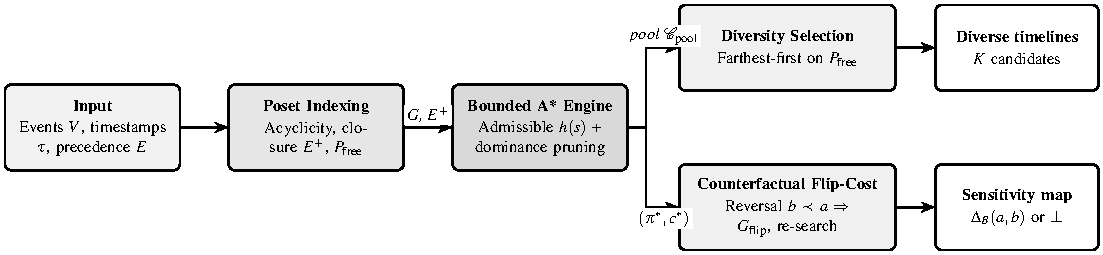
\includegraphics[width=\textwidth]{figures/arch.pdf}
\caption{Architecture of the counterfactual flip-cost framework. Events, timestamps, and precedence constraints are indexed as a poset; a bounded A* engine with an admissible heuristic and dominance pruning produces an optimal timeline $\pi^*$ and a candidate pool, which branch into (i) farthest-first diversity selection over $\Pfree$ and (ii) counterfactual flip-cost evaluation producing the pairwise sensitivity map $\Delta_B$.}
\label{fig:arch}
\end{figure*}

\subsection{Ingestion and Reachability Precomputation}
Acyclicity of $G$ is verified by topological sort in $O(|V|+|E|)$ time \cite{Tarjan1972,Cormen2022}; a detected cycle indicates inconsistent constraints and terminates execution. The transitive closure is computed by repeated traversals in $O(|V|(|V|+|E|))$, caching $\mathrm{Anc}(v)$ and $\mathrm{Desc}(u)$ for $O(1)$ reachability queries. Then $\Pfree=\{(u,v)\mid u<v,\ v\notin\mathrm{Desc}(u),\ u\notin\mathrm{Desc}(v)\}$.

\subsection{Bounded A* with Dominance Pruning}
A search state is $s=(P,U,R)$: an ordered prefix $P$, its vertex set $U$, and the remaining set $R=V\setminus U$. A vertex $w\in R$ is an admissible successor iff $\mathrm{Pred}_G(w)\subseteq U$. The priority is $f(s)=g(s)+h(s)$, where $g(s)$ is the exact inversion cost of the prefix, updated incrementally by
\begin{equation}
\Delta g(P,w)=\sum_{u\in P}\ind[\pos_{\pi_\tau}(u)>\pos_{\pi_\tau}(w)].
\end{equation}
For any $u,v\in R$ with $(u,v)\in E^+$, every completion must place $u$ before $v$; if $u$ has the later timestamp, the pair is a guaranteed inversion. Hence
\begin{equation}
h(s)=\sum_{\substack{u,v\in R\\ u\neq v}}\ind\big[(u,v)\in E^+\wedge\pos_{\pi_\tau}(u)>\pos_{\pi_\tau}(v)\big].
\end{equation}

\begin{theorem}[Admissibility of $h$]\label{thm:adm}
$h(s)$ never overestimates the minimum additional cost $h^*(s)$ of completing prefix $P$: $0\le h(s)\le h^*(s)$. Moreover, $h(s)$ depends on $s$ only through $U$.
\end{theorem}
\begin{proof}
Let $\pi$ be any valid completion of $P$. It places $R$ in positions $m+1,\dots,n$. For $u,v\in R$ with $(u,v)\in E^+$, validity gives $\pos_\pi(u)<\pos_\pi(v)$; if $\pos_{\pi_\tau}(u)>\pos_{\pi_\tau}(v)$ this pair is discordant by definition and contributes one inversion to $c(\pi)$. These pairs lie entirely inside $R$, so they are disjoint from the inversions already counted in $g(s)$ (pairs inside $U$ or between $U$ and $R$). Thus $c(\pi)-g(s)\ge h(s)$ for every completion, so $h(s)\le h^*(s)$. Because $R=V\setminus U$, $h$ is a function of $U$ alone.
\end{proof}

\emph{Remark.} $h$ is admissible but is not guaranteed to be consistent: expanding $w$ removes from $h$ the forced inversions involving $w$ while $\Delta g(P,w)$ counts only inversions against placed events. Optimality is nevertheless preserved, because (i) A* with an admissible heuristic returns an optimal solution when a goal is first popped (at a goal $h=0$ and $f=c$), and (ii) pruning is based on Lemma~\ref{lem:dom}, which relies only on the fact that $h$ depends on $U$ alone, not on consistency.

\begin{lemma}[Prefix dominance]\label{lem:dom}
Let $s_1=(P_1,U,R)$ and $s_2=(P_2,U,R)$ share the same placed set $U$. For every $w\in R$, $\Delta g(P_1,w)=\Delta g(P_2,w)$. Consequently, if $g(s_1)\le g(s_2)$, then $s_2$ can be pruned without loss of optimality.
\end{lemma}
\begin{proof}
For $w\in R$, an inversion with $u\in U$ occurs iff $\pos_{\pi_\tau}(u)>\pos_{\pi_\tau}(w)$. The set $\{u\in U:\pos_{\pi_\tau}(u)>\pos_{\pi_\tau}(w)\}$ depends on the membership of $U$, not on the internal permutation of $P_1$ or $P_2$, because every element of $U$ precedes every element of $R$ in any completion. The same argument applies to every pair of $U$ and $R$, so for any completion $\pi_R$ of $R$, the cross-inversions between $U$ and $R$ and the inversions within $R$ are identical under $P_1$ and $P_2$: $c(P_1\circ\pi_R)-g(s_1)=c(P_2\circ\pi_R)-g(s_2)$. If $g(s_1)\le g(s_2)$ then $c(P_1\circ\pi_R)\le c(P_2\circ\pi_R)$ for all $\pi_R$, so $s_2$ cannot yield a strictly better solution.
\end{proof}


\begin{figure}[!t]
\centering
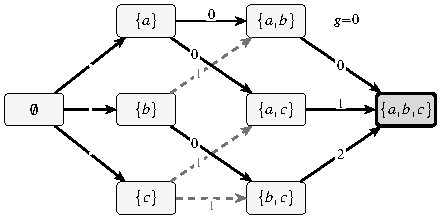
\includegraphics[width=\columnwidth]{figures/dominance.pdf}
\caption{Subset-dominance pruning (Lemma~\ref{lem:dom}) for three unconstrained events with $\tau(a)<\tau(b)<\tau(c)$. Edge labels are $\Delta g(P,w)$. The prefixes $(a,b)$ and $(b,a)$ reach the same placed set $\{a,b\}$ with $g=0$ and $g=1$, so the dashed branch is pruned; only one best prefix per subset is kept, so the search explores at most $2^{|V|}$ subsets rather than $|V|!$ orderings.}
\label{fig:dominance}
\end{figure}

Fig.~\ref{fig:dominance} shows the effect of Lemma~\ref{lem:dom} on a toy instance.

\begin{algorithm}[!t]
\caption{Bounded A* with Dominance Pruning}\label{alg:astar}
\footnotesize
\begin{algorithmic}[1]
\Require DAG $G=(V,E)$, reference order $\pi_\tau$, budget $B$, pool size $K$
\Ensure \textsc{Result}(timeline, cost, expansions, status, pool)
\State $\mathit{Open}\gets$ priority queue; $\mathit{BestG}[\emptyset]\gets 0$
\State push $(h(V),\,0,\,0,\,(\,),\,V)$ onto $\mathit{Open}$; $\mathit{Done}\gets[\,]$; $x\gets 0$
\While{$\mathit{Open}\neq\emptyset$ \textbf{and} $x<B$}
  \State pop $(f,\cdot,g,P,R)$; $U\gets\mathrm{set}(P)$
  \If{$|P|<|V|$ \textbf{and} $g>\mathit{BestG}[U]$} \textbf{continue} \Comment{dominated}
  \EndIf
  \If{$|P|=|V|$}
    \State append $(g,P)$ to $\mathit{Done}$
    \If{$|\mathit{Done}|\ge K$} \State sort $\mathit{Done}$ by cost; \Return $(\mathit{Done}[0],x,\textsc{Exact})$
    \EndIf
    \State \textbf{continue}
  \EndIf
  \State $x\gets x+1$
  \State $A\gets\{w\in R:\mathrm{Pred}_G(w)\subseteq U\}$, sorted by $\pos_{\pi_\tau}(w)$
  \For{$w\in A$}
    \State $P'\gets P\circ w$; $U'\gets U\cup\{w\}$; $R'\gets R\setminus\{w\}$
    \State $g'\gets g+\Delta g(P,w)$
    \If{$|P'|<|V|$}
      \If{$g'\ge\mathit{BestG}[U']$} \textbf{continue} \Comment{dominated successor}
      \EndIf
      \State $\mathit{BestG}[U']\gets g'$
    \EndIf
    \State push $(g'+h(R'),\,-|P'|,\,g',\,P',\,R')$ onto $\mathit{Open}$
  \EndFor
\EndWhile
\If{$\mathit{Done}\neq\emptyset$}
  \State sort $\mathit{Done}$; \Return $(\mathit{Done}[0],x,\textsc{Feasible})$
\Else
  \State \Return $(\mathrm{None},x,\textsc{BudgetExhausted})$
\EndIf
\end{algorithmic}
\end{algorithm}

Algorithm~\ref{alg:astar} implements this search. The status is \textsc{Exact} when $K$ complete timelines are popped (the first popped is optimal by Theorem~\ref{thm:adm}), \textsc{Feasible} when the budget ends after at least one completion, and \textsc{BudgetExhausted} otherwise.

\subsection{Diversity-Aware Candidate Selection}
Top-$K$ search tends to return timelines differing only by swaps of independent background events. For $\pi_i,\pi_j\in\Lin(G)$ we define the normalized free-pair disagreement
\begin{multline}
\dfree(\pi_i,\pi_j)=\frac{1}{|\Pfree|}\sum_{(u,v)\in\Pfree}\ind\big[(\pos_{\pi_i}(u)<\pos_{\pi_i}(v))\\
\neq(\pos_{\pi_j}(u)<\pos_{\pi_j}(v))\big],
\end{multline}
with $\dfree=0$ if $\Pfree=\emptyset$. Algorithm~\ref{alg:div} selects $K$ candidates from the pool by farthest-first traversal.

\begin{algorithm}[!t]
\caption{Diversity-Aware Farthest-First Selection}\label{alg:div}
\footnotesize
\begin{algorithmic}[1]
\Require pool $\mathcal{C}_{\mathrm{pool}}$ sorted by cost, target $K$, free pairs $\Pfree$
\Ensure diverse set $S$
\If{$|\mathcal{C}_{\mathrm{pool}}|\le K$} \Return $\mathcal{C}_{\mathrm{pool}}$
\EndIf
\State $S\gets[\mathcal{C}_{\mathrm{pool}}[0]]$; $\mathit{Rem}\gets\mathcal{C}_{\mathrm{pool}}[1{:}]$
\While{$|S|<K$ \textbf{and} $\mathit{Rem}\neq\emptyset$}
  \State $\mathit{best}\gets\mathrm{None}$; $\mu^*\gets-1$
  \For{each $c\in\mathit{Rem}$}
    \State $\mu\gets\min_{s\in S}\dfree(c,s)$
    \If{$\mu>\mu^*$} \State $\mu^*\gets\mu$; $\mathit{best}\gets c$
    \EndIf
  \EndFor
  \State append $\mathit{best}$ to $S$; remove it from $\mathit{Rem}$
\EndWhile
\State \Return $S$
\end{algorithmic}
\end{algorithm}

\subsection{Counterfactual Flip-Cost Evaluation}
Algorithm~\ref{alg:flip} evaluates a free pair $(u,v)$ by orienting it according to $\pi^*$, adding the reversal edge, and re-running Algorithm~\ref{alg:astar}.

\begin{algorithm}[!t]
\caption{Counterfactual Flip-Cost $\Delta_B(a,b)$}\label{alg:flip}
\footnotesize
\begin{algorithmic}[1]
\Require DAG $G$, baseline result $(\pi^*,c^*)$, pair $(u,v)\in\Pfree$, budget $B$
\Ensure \textsc{FlipResult}(pair, $\Delta$, status)
\If{$\pi^*=\mathrm{None}$} \Return \textsc{Failure}
\EndIf
\If{$\pos_{\pi^*}(u)<\pos_{\pi^*}(v)$} $(a,b)\gets(u,v)$ \textbf{else} $(a,b)\gets(v,u)$
\EndIf
\If{$(a,b)\in E^+$} \Return $(\,(a,b),\mathrm{None},\textsc{Infeasible})$ \Comment{reversal causally impossible}
\EndIf
\State $G_{\mathrm{flip}}\gets(V,E\cup\{(b,a)\})$
\State $R\gets\textsc{BoundedAStar}(G_{\mathrm{flip}},\pi_\tau,B,1)$
\If{$R.\mathrm{status}\in\{\textsc{Exact},\textsc{Feasible}\}$}
  \State \Return $(\,(a,b),\,R.\mathrm{cost}-c^*,\,R.\mathrm{status})$
\Else
  \State \Return $(\,(a,b),\,\bot,\,\textsc{BudgetExhausted})$
\EndIf
\end{algorithmic}
\end{algorithm}

\subsection{Asymptotic Complexity}
Preprocessing costs $O(|V|(|V|+|E|))$ for closure and $O(|V|^2)$ for $\Pfree$. With at most $S\le B$ expansions, each costing $O(|V|)$ for successors and incremental cost (the heuristic is maintained incrementally via per-vertex forced-inversion counts) plus $O(\log S)$ per heap push, a single search costs $O(S(|V|+\log S))$ time and $O(S|V|)$ space. Farthest-first selection over a pool of size $M$ costs $O(KM|\Pfree|)$. Evaluating all free pairs requires $|\Pfree|$ bounded searches:
\begin{equation}
T_{\mathrm{total}}=O\big(|\Pfree|\cdot B\cdot(|V|+\log B)\big).
\end{equation}
Analysts may restrict evaluation to pairs implicated in critical attack stages for targeted triage.

%=====================================================================
\section{Experimental Setup}\label{sec:setup}
All experiments ran on an AMD Ryzen-class machine with Python 3.11 (\texttt{numpy}, \texttt{scipy}, \texttt{networkx}, \texttt{scikit-learn}). All benchmarking code, synthetic poset generators, noise distortion models, and unit test suites are open-sourced for reproducibility at \url{https://github.com/Disgusting-Orange/counterfactual-flip-cost}.

\subsection{Benchmark Generation}
Verified microsecond-level ground truth is unavailable for real incidents, so we use synthetic posets with known ground truth. A true sequence $\pi_{\mathrm{true}}$ of $n$ events is generated with inter-event gaps $\Delta t_i\sim\mathrm{Exp}(\lambda=0.5)$. Precedence edges are sampled with density $p_{\mathrm{edge}}\in[0.15,0.35]$ consistent with $\pi_{\mathrm{true}}$, guaranteeing acyclicity and $\pi_{\mathrm{true}}\in\Lin(G)$. Sizes range from $n=10$ to $50$; small instances $n\in\{7,\dots,10\}$ are checked against brute force over all $n!$ permutations.

\subsection{Noise Models}
To avoid circularity between noise generation and the inversion objective, we use two distinct models.

\emph{Noise Model 1 (Gaussian jitter and missing records):}
\begin{equation}
\tau(v)=\max\big(0,\ t_{\mathrm{true}}(v)+\mathcal{N}(0,\sigma^2)+\delta_{\mathrm{burst}}(v)\big),
\end{equation}
with $\sigma\in\{1.0,1.5,2.0,4.0\}$\,s, delay bursts $\delta_{\mathrm{burst}}\sim\mathcal{U}(3,8)$\,s with probability $0.10$, and missing records at rate $\le0.30$.

\emph{Noise Model 2 (structured multi-source clock skew, after \cite{Kimm2026}):} events are spread over $M=4$ hosts, each with static offset $\Delta_m\sim\mathcal{U}(-4,4)$\,s and drift $\alpha_m\sim\mathcal{N}(0,0.05)$, and timestamps are quantised to 1.0\,s:
\begin{equation}
\tau(v)=\mathrm{round}\!\Big(\frac{t_{\mathrm{true}}(v)+\Delta_m+\alpha_m t_{\mathrm{true}}(v)}{\Delta_{\mathrm{quant}}}\Big)\Delta_{\mathrm{quant}}.
\end{equation}
This yields non-monotonic arrivals and identical timestamps, mimicking EVTX and Syslog distortions.


\begin{figure}[!t]
\centering
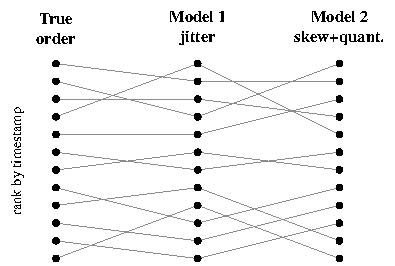
\includegraphics[width=0.72\columnwidth]{figures/noise.pdf}
\caption{Illustrative realization of the two noise models on 12 events (fixed seed). Each line follows one event from its true rank (left) to its rank under Gaussian jitter with bursts (centre, $\sigma=1.5$\,s) and under four-host clock skew with 1\,s quantisation (right). Line crossings are timestamp-induced inversions: 9 discordant pairs for Model 1 and 5 for Model 2 relative to the true order. Under such distortion the recorded order $\pi_\tau$ is generally not a linear extension of $G$.}
\label{fig:noise}
\end{figure}

Fig.~\ref{fig:noise} visualizes both models.

\subsection{Baselines}
We compare $\Delta_B(a,b)$ with: (i) the \textbf{timestamp margin} $|\tau(b)-\tau(a)|$; and (ii) a \textbf{Mallows marginal} baseline in the style of process-mining estimators \cite{vanderAa2020,Pegoraro2021}, computed over the candidate pool $\mathcal{C}_{\mathrm{pool}}$ with $\theta=0.5$:
\begin{equation}
P(a\prec b)=\frac{\sum_{\pi\in\mathcal{C}_{\mathrm{pool}}:\ \pos_\pi(a)<\pos_\pi(b)}e^{-\theta c(\pi)}}{\sum_{\pi\in\mathcal{C}_{\mathrm{pool}}}e^{-\theta c(\pi)}}.
\end{equation}

\subsection{Metrics}
\emph{Validity} (\% of returned timelines satisfying all edges); \emph{diversity} $\dfree$ (mean pairwise distance on $\Pfree$); \emph{mean cost} $c(\pi)$; \emph{union coverage} (fraction of free pairs for which at least one candidate matches the ground-truth relative order); \emph{expansions} $S$ and \emph{runtime} (ms); and \emph{AUROC} of each sensitivity score in discriminating correct ($y=1$) from inverted ($y=0$) pairwise decisions, with paired 95\% bootstrap confidence intervals over 1{,}000 resamples.

%=====================================================================
\section{Results and Discussion}\label{sec:results}

\subsection{Exactness Verification}
On 60 independently seeded instances with $n\in\{7,8,9,10\}$, where the $n!$ permutation space can be enumerated, Algorithm~\ref{alg:astar} matched the brute-force global minimum cost in 100\% of cases (60/60). This empirically supports the admissibility of $h$ (Theorem~\ref{thm:adm}) and the safety of subset-dominance pruning (Lemma~\ref{lem:dom}).

\subsection{Candidate Selection: Diversity versus Cost}
Table~\ref{tab:select} compares three strategies at $N=18$, $K=5$, $\sigma=1.5$, $B=1000$: score-only best-first, pool-based farthest-first selection, and flip-based diversity.

\begin{table}[!t]
\caption{Candidate Selection Under Gaussian Jitter ($N=18$, $K=5$, $\sigma=1.5$)}
\label{tab:select}
\centering
\footnotesize
\setlength{\tabcolsep}{3.5pt}
\renewcommand{\arraystretch}{1.1}
\begin{tabular}{@{}lrrr@{}}
\toprule
\textbf{Metric} & \textbf{Score-Only} & \textbf{Pool+Div.} & \textbf{Flip-Div.}\\
\midrule
Validity (\%) & 100 & 100 & 100\\
Diversity $\dfree$ & 0.060 & 0.077 & 0.145\\
Mean cost & 5.59 & 6.26 & 8.41\\
Union coverage & 0.927 & 0.930 & 0.948\\
Expansions $S$ & 546.7 & 546.7 & 2186.7\\
Runtime (ms) & 16.3 & 16.6 & 52.3\\
\bottomrule
\end{tabular}
\end{table}

All strategies were 100\% valid. Score-only selection yields low diversity (0.060) because top candidates differ by trivial local swaps. Pool-based farthest-first selection raises diversity to 0.077 (+28.3\%) at negligible overhead (+0.3\,ms) and slightly raises coverage (0.927 to 0.930). Forcing counterfactual flips during candidate generation raises diversity to 0.145 (+141.7\%) and coverage to 0.948, but increases mean cost from 5.59 to 8.41 and requires about four times the expansions (2186.7) and 52.3\,ms. Fig.~\ref{fig:pareto} shows this explicit trade-off: analysts seeking broader hypothesis coverage can widen the search at the price of higher sub-optimality.

\begin{figure}[!t]
\centering
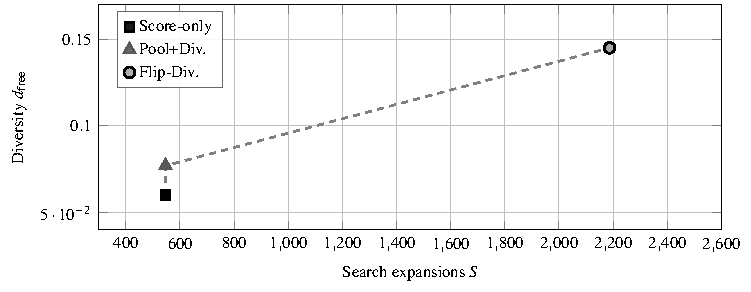
\includegraphics[width=\columnwidth]{figures/pareto.pdf}
\caption{Diversity--effort trade-off ($N=18$, $K=5$, $\sigma=1.5$): free-pair diversity $d_{\mathrm{free}}$ versus search expansions for the three selection strategies. Pool-based selection improves diversity at no extra expansions; flip-based diversity reaches the highest diversity at roughly four times the expansions.}
\label{fig:pareto}
\end{figure}

\subsection{Sensitivity AUROC}
Table~\ref{tab:auroc} reports AUROC across noise scales and models, Fig.~\ref{fig:auroc} plots the Gaussian settings and Fig.~\ref{fig:forest} the paired differences against the margin baseline.

\begin{table*}[!t]
\caption{Pairwise Sensitivity AUROC Across Noise Scales and Models}
\label{tab:auroc}
\centering
\footnotesize
\setlength{\tabcolsep}{6pt}
\renewcommand{\arraystretch}{1.1}
\begin{tabular}{@{}llcccc@{}}
\toprule
\textbf{Noise model} & \textbf{Setting} & \textbf{Flip-cost $\Delta$} & \textbf{Margin $|\Delta\tau|$} & \textbf{Mallows $P(a\prec b)$} & \textbf{Paired diff. [95\% CI] (Flip $-$ Margin)}\\
\midrule
Gaussian jitter & $\sigma=1.0$ & 0.856 & 0.855 & 0.593 & $+0.002$ [$-0.024$, $+0.028$]\\
Gaussian jitter & $\sigma=1.5$ & 0.849 & 0.856 & 0.585 & $-0.007$ [$-0.029$, $+0.014$]\\
Gaussian jitter & $\sigma=2.0$ & 0.832 & 0.847 & 0.595 & $-0.014$ [$-0.037$, $+0.007$]\\
Gaussian jitter & $\sigma=4.0$ & 0.801 & 0.740 & 0.583 & $+0.061$ [$+0.030$, $+0.092$]$^{*}$\\
\midrule
Structured clock skew & 4 hosts, offsets $\pm4$\,s & 0.835 & 0.830 & 0.605 & $+0.006$ [$-0.021$, $+0.031$]\\
\bottomrule
\multicolumn{6}{l}{$^{*}$Statistically significant ($p<0.001$): paired bootstrap interval excludes zero.}
\end{tabular}
\end{table*}

\begin{figure}[!t]
\centering
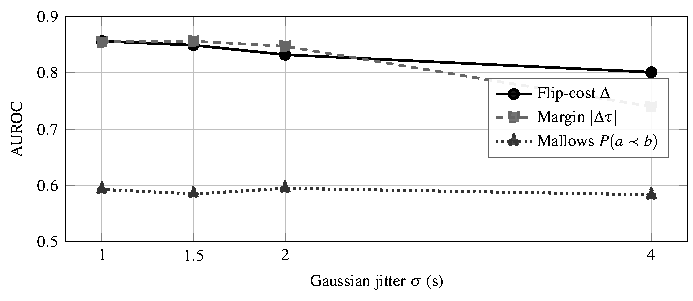
\includegraphics[width=\columnwidth]{figures/auroc.pdf}
\caption{Sensitivity AUROC versus Gaussian jitter $\sigma$ for counterfactual flip-cost, timestamp margin, and Mallows marginal probability. Flip-cost matches the margin at low noise and clearly exceeds it at $\sigma=4$\,s; the Mallows marginal remains near 0.58--0.60 throughout.}
\label{fig:auroc}
\end{figure}


\begin{figure}[!t]
\centering
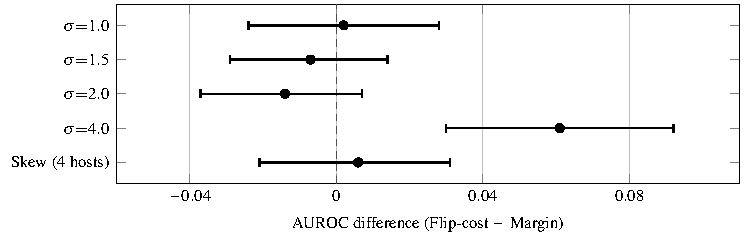
\includegraphics[width=\columnwidth]{figures/forest.pdf}
\caption{Paired AUROC difference between flip-cost and the timestamp margin with 95\% bootstrap intervals (1,000 resamples; Table~\ref{tab:auroc}). Intervals cross zero in four of five settings; only $\sigma=4$\,s excludes zero.}
\label{fig:forest}
\end{figure}

\emph{Why the marginal fails.} Across all settings the Mallows marginal baseline attains only 0.583--0.605 AUROC. In a single-incident poset with high combinatorial flexibility, marginals over a bounded pool concentrate near 0.5 for free pairs and cannot separate correct from inverted orderings. The flip-cost, an extremal quantity (Theorem~\ref{thm:map}), reaches 0.801--0.856.

\emph{Robustness under severe noise.} For $\sigma\le2.0$\,s, flip-cost and margin are statistically indistinguishable (all paired intervals include zero). At $\sigma=4.0$\,s, the margin collapses to 0.740 while flip-cost retains 0.801; the paired difference of $+0.061$ has 95\% CI $[+0.030,+0.092]$, excluding zero. Under heavy distortion, raw time gaps mislead, while the topological constraints enforced during the counterfactual search preserve discriminative power. Under the structured multi-host skew model, flip-cost (0.835) is on par with the margin (0.830; difference $+0.006$, CI includes zero) and far above the marginal baseline (0.605), indicating the behavior is not specific to Gaussian noise.

\subsection{Computational Scalability}
Table~\ref{tab:scale} and Fig.~\ref{fig:scale} summarize scalability of Algorithm~\ref{alg:astar} at $B=3000$.

\begin{table}[!t]
\caption{Scalability of Bounded A* ($B=3000$)}
\label{tab:scale}
\centering
\footnotesize
\setlength{\tabcolsep}{6pt}
\renewcommand{\arraystretch}{1.1}
\begin{tabular}{@{}rrrr@{}}
\toprule
\textbf{Events $N$} & \textbf{Runtime (ms)} & \textbf{Expansions $S$} & \textbf{Mean cost}\\
\midrule
10 & 0.93 & 83.7 & 1.73\\
20 & 7.63 & 305.0 & 4.33\\
30 & 45.84 & 914.5 & 5.91\\
40 & 231.12 & 1681.0 & 10.09\\
50 & 327.37 & 1530.3 & 11.44\\
\bottomrule
\end{tabular}
\end{table}

\begin{figure}[!t]
\centering
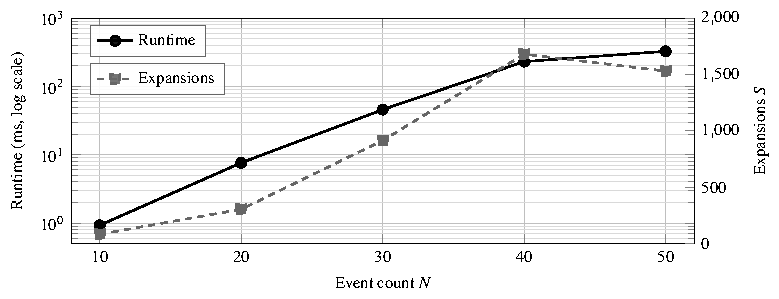
\includegraphics[width=\columnwidth]{figures/scale.pdf}
\caption{Computational scalability from $N=10$ to $50$ events at $B=3000$: mean runtime (left axis, logarithmic) and mean search expansions (right axis, linear).}
\label{fig:scale}
\end{figure}

Even at $N=50$, where the unconstrained permutation space has $50!\approx3.04\times10^{64}$ elements, the admissible heuristic and subset-dominance pruning limit the search to about 1{,}530 expansions and 327\,ms, which is compatible with interactive use in SOC consoles for a single baseline search. Total flip analysis multiplies this by the number of evaluated pairs (Section~\ref{sec:method}).

%=====================================================================
\section{Threats to Validity and Limitations}\label{sec:threats}

\subsection{Construct Validity}
\emph{Objective proxy.} The cost $c(\pi)$ measures agreement with recorded timestamps; it is an objective-relative metric, not a guarantee of historical truth. If timestamps are systematically forged over an interval, the optimizer will faithfully fit the forged data. Flip-cost quantifies stability of a decision \emph{with respect to this objective}, not ontological causal ground truth.

\emph{Poset under-specification.} For $(a,b)\in\Pfree$, neither order is physically invalid. A pairwise ``error'' against $\pi_{\mathrm{true}}$ may therefore reflect missing domain constraints rather than a reconstruction failure.

\subsection{Internal Validity}
\emph{Budget ceilings.} If the budget $B$ is exhausted before a feasible counterfactual extension is found, the result is $\bot$ and must never be read as $\Delta=\infty$; deployments must tune $B$ against latency requirements.

\emph{Dispersion $\theta$.} The Mallows baseline depends on $\theta$; single-incident data cannot fit $\theta$ by maximum likelihood, and our sensitivity checks over $\theta\in[0.1,1.0]$ do not remove this limitation. Note that $\Delta$ itself is independent of $\theta$ (Theorem~\ref{thm:map}).

\subsection{External Validity}
Our evaluation uses synthetic DAGs with the multi-host skew model of \cite{Kimm2026}. Validity on operational feeds (e.g., DARPA OpTC and Windows Sysmon traces) remains to be established, and extracting fine-grained causal DAGs from noisy audit streams depends on provenance pipelines such as \cite{Hossain2017,Cheng2024}.

%=====================================================================
\section{Conclusion and Future Work}\label{sec:conclusion}
We introduced counterfactual flip-cost analysis to quantify pairwise ordering ambiguity in precedence-constrained security timelines. We cast reconstruction as constrained Kendall-tau minimization (NP-complete), proved that $\Delta(a,b)$ equals the scaled log-ratio of extremal MAP realizations under a precedence-conditioned Mallows model, and developed a budget-bounded A* search with an admissible heuristic and exact dominance pruning, plus farthest-first diversity selection over $\Pfree$. Experiments showed 100\% agreement with brute force (60/60), scaling to $N=50$ in 327\,ms, flip-cost AUROC of 0.801--0.856 versus 0.583--0.605 for the Mallows marginal, and a statistically significant advantage over the timestamp margin at $\sigma=4$\,s ($+0.061$, 95\% CI $[+0.030,+0.092]$).

Future work will: (i) validate on DARPA OpTC and DARPA Transparent Computing data; (ii) reuse priority-queue state between baseline and counterfactual searches to reduce the cost of full flip analysis from $O(|\Pfree|\cdot B)$ toward near-constant incremental updates; and (iii) integrate flip-cost heatmaps into SIEM consoles to give investigators interactive sensitivity indicators during triage.


\balance
\begin{thebibliography}{30}
\bibitem{vanderAa2020} H. van der Aa, H. Leopold, and M. Weidlich, ``Partial order resolution of event logs for process conformance checking,'' \emph{Decision Support Systems}, vol. 136, Art. no. 113347, 2020, doi: 10.1016/j.dss.2020.113347.

\bibitem{Lepsien2024} A. Lepsien, M. Pegoraro, F. Fonger, D. Langhammer, M. Aleknyte-Resch, and A. Koschmider, ``Ranking the top-$K$ realizations of stochastically known event logs,'' in \emph{Process Mining Workshops (ICPM 2024)}, LNBIP, vol. 533. Springer, 2025, pp. 350--362, doi: 10.1007/978-3-031-82225-4\_26.

\bibitem{Aljazzar2011} H. Aljazzar and S. Leue, ``$K^*$: A heuristic search algorithm for finding the $k$ shortest paths,'' \emph{Artificial Intelligence}, vol. 175, no. 18, pp. 2129--2154, 2011, doi: 10.1016/j.artint.2011.07.003.

\bibitem{Eppstein1998} D. Eppstein, ``Finding the $k$ shortest paths,'' \emph{SIAM J. Comput.}, vol. 28, no. 2, pp. 652--673, 1998, doi: 10.1137/S0097539795290477.

\bibitem{Hossain2017} M. N. Hossain, S. M. Milajerdi, J. Wang, B. Eshete, R. Gjomemo, R. Sekar, S. Stoller, and V. N. Venkatakrishnan, ``SLEUTH: Real-time attack scenario reconstruction from COTS audit data,'' in \emph{Proc. 26th USENIX Security Symp. (USENIX Security 17)}, 2017, pp. 487--504.

\bibitem{Cheng2024} Z. Cheng, Q. Lv, J. Liang, Y. Wang, D. Sun, T. Pasquier, and X. Han, ``KAIROS: Practical intrusion detection and investigation using whole-system provenance,'' in \emph{Proc. 45th IEEE Symp. Security and Privacy (S\&P)}, 2024, pp. 1243--1260, doi: 10.1109/SP54263.2024.00072.

\bibitem{Kimm2026} H. Kimm, S. Mishra, and R. Sekar, ``Minding the gap: Bridging causal disconnects in system provenance,'' in \emph{Proc. Network and Distributed System Security Symp. (NDSS / PRISM)}, 2026, doi: 10.14722/prism.2026.23023.

\bibitem{Peisert2007} S. Peisert, M. Bishop, S. Karin, and K. Marzullo, ``Analysis of computer intrusions using sequences of system calls,'' \emph{IEEE Trans. Dependable Secure Comput.}, vol. 4, no. 2, pp. 137--150, Apr.--Jun. 2007.

\bibitem{Pegoraro2020a} M. Pegoraro, M. S. Uysal, and W. M. P. van der Aalst, ``Efficient time and space representation of uncertain event data,'' \emph{Algorithms}, vol. 13, no. 11, Art. no. 285, 2020, doi: 10.3390/a13110285.

\bibitem{Brightwell1991} G. Brightwell and P. Winkler, ``Counting linear extensions,'' \emph{Order}, vol. 8, no. 3, pp. 225--242, 1991, doi: 10.1007/BF00383444.

\bibitem{Brandenburg2011} F. J. Brandenburg, A. Glei{\ss}ner, and A. Hofmeier, ``Comparing and aggregating partial orders with Kendall tau distances,'' Univ. Passau, Passau, Germany, Tech. Rep. MIP-1102, 2011.

\bibitem{Pegoraro2021} M. Pegoraro, B. Bakullari, M. S. Uysal, and W. M. P. van der Aalst, ``Probability estimation of uncertain process trace realizations,'' in \emph{Proc. Int. Conf. Business Information Systems (BIS)}, LNBIP, vol. 444. Springer, 2021, pp. 18--30.

\bibitem{Lu2011} T. Lu and C. Boutilier, ``Learning Mallows models with pairwise preferences,'' in \emph{Proc. 28th Int. Conf. Machine Learning (ICML)}, 2011, pp. 145--152.

\bibitem{Pegoraro2020b} M. Pegoraro, M. S. Uysal, and W. M. P. van der Aalst, ``Efficient construction of behavior graphs for uncertain event data,'' in \emph{Proc. 23rd Int. Conf. Business Information Systems (BIS)}, LNBIP, vol. 389. Springer, 2020, pp. 76--88.

\bibitem{Dittmer2020} S. Dittmer and I. Pak, ``Counting linear extensions of restricted posets,'' \emph{Electron. J. Combinatorics}, vol. 27, no. 4, Art. no. P4.48, 2020.

\bibitem{Kangas2016} K. Kangas, T. Hankala, T. Niinim{\"a}ki, and M. Koivisto, ``Counting linear extensions of sparse posets,'' in \emph{Proc. 25th Int. Joint Conf. Artificial Intelligence (IJCAI)}, 2016, pp. 603--609.

\bibitem{Huber2006} M. Huber, ``Fast perfect sampling from linear extensions,'' \emph{Discrete Math.}, vol. 306, no. 4, pp. 420--428, 2006, doi: 10.1016/j.disc.2005.12.016.

\bibitem{vanZuylen2009} A. van Zuylen and D. P. Williamson, ``Deterministic pivoting algorithms for constrained ranking and clustering problems,'' \emph{Math. Oper. Res.}, vol. 34, no. 3, pp. 594--620, 2009, doi: 10.1287/moor.1090.0384.

\bibitem{Sohrabi2016} S. Sohrabi, A. V. Riabov, O. Udrea, and O. Hassanzadeh, ``Finding diverse high-quality plans for hypothesis generation,'' in \emph{Proc. 22nd Eur. Conf. Artificial Intelligence (ECAI)}, 2016, pp. 1581--1582.

\bibitem{Batra2012} D. Batra, P. Yadollahpour, A. Guzman-Rivera, and G. Shakhnarovich, ``Diverse $M$-best solutions in Markov random fields,'' in \emph{Proc. Eur. Conf. Computer Vision (ECCV)}, LNCS, vol. 7576. Springer, 2012, pp. 1--16.

\bibitem{Katz2020} M. Katz, S. Sohrabi, and O. Udrea, ``Top-quality planning: Finding practically useful sets of best plans,'' in \emph{Proc. 34th AAAI Conf. Artificial Intelligence}, vol. 34, no. 6, 2020, pp. 9900--9907.

\bibitem{Katz2022} M. Katz, S. Sohrabi, and O. Udrea, ``Bounding quality in diverse planning,'' in \emph{Proc. 36th AAAI Conf. Artificial Intelligence}, vol. 36, no. 9, 2022, pp. 9805--9812.

\bibitem{Wachter2018} S. Wachter, B. Mittelstadt, and C. Russell, ``Counterfactual explanations without opening the black box: Automated decisions and the GDPR,'' \emph{Harvard J. Law \& Technol.}, vol. 31, no. 2, pp. 841--887, 2018.

\bibitem{King2003} S. T. King and P. M. Chen, ``Backtracking intrusions,'' in \emph{Proc. 19th ACM Symp. Operating Systems Principles (SOSP)}, 2003, pp. 223--236.

\bibitem{Pasquier2017} T. Pasquier, X. Han, M. Goldstein, T. Kohno, M. Seltzer, and J. Singh, ``Practical whole-system provenance capture,'' in \emph{Proc. ACM Symp. Cloud Computing (SoCC)}, 2017, pp. 405--418.

\bibitem{Kendall1938} M. G. Kendall, ``A new measure of rank correlation,'' \emph{Biometrika}, vol. 30, no. 1/2, pp. 81--93, 1938.

\bibitem{Mallows1957} C. L. Mallows, ``Non-null ranking models. I,'' \emph{Biometrika}, vol. 44, no. 1/2, pp. 114--130, 1957.

\bibitem{Mastrolilli2011} M. Mastrolilli, ``The feedback arc set problem with triangle inequality is a vertex cover problem,'' \emph{CoRR}, vol. abs/1111.4299, 2011.

\bibitem{Cormen2022} T. H. Cormen, C. E. Leiserson, R. L. Rivest, and C. Stein, \emph{Introduction to Algorithms}, 4th ed. Cambridge, MA, USA: MIT Press, 2022.

\bibitem{Tarjan1972} R. E. Tarjan, ``Depth-first search and linear graph algorithms,'' \emph{SIAM J. Comput.}, vol. 1, no. 2, pp. 146--160, 1972.
\end{thebibliography}




\begin{IEEEbiography}[{}]{Kamalesh N.} is currently pursuing the B.Tech. degree in Computer Science and Engineering at the Vellore Institute of Technology (VIT), Chennai, India. His research interests include digital forensics, system provenance, graph algorithms, and incident timeline reconstruction.
\end{IEEEbiography}
\begin{IEEEbiography}[{}]{Varun Dubey} is currently pursuing the B.Tech. degree in Computer Science and Engineering at the Vellore Institute of Technology (VIT), Chennai, India. His research interests include heuristic search, combinatorial optimization, and algorithm design.
\end{IEEEbiography}

\EOD

\end{document}
